\documentclass[11pt]{article}
\usepackage[margin=1in]{geometry}
\usepackage{times}
\usepackage{latexsym}
\usepackage{graphicx}
\usepackage{booktabs}
\usepackage{hyperref}
\usepackage{amsmath}
\usepackage{fancyhdr}
\usepackage{lastpage}
\usepackage{subcaption}
\usepackage{xcolor}
\usepackage{float}
\usepackage{fancyvrb}

% Title and Author
\title{CSE 240A Branch Predictor Project:\\
G-Share, Tournament, and a Custom TAGE Implementation}

\author{%
  Param Somane \\
  Department of Computer Science and Engineering \\
  University of California, San Diego \\
  \texttt{psomane@ucsd.edu}
}

\date{May 29, 2025}


% For final wrap-up
\fancypagestyle{ack_footer}{
    \fancyhf{}
    \renewcommand{\headrulewidth}{0pt}
    \renewcommand{\footrulewidth}{0pt}
    \cfoot{
      \scriptsize
      \begin{minipage}[t]{0.95\textwidth}
      \textbf{AI Acknowledgments:} OpenAI's ChatGPT (model gpt-4o) was utilized to generate code from formulas and algorithms, assist in generating the visualization script to create plots from results, adding comments where needed, to help debug code and set up errors, and assist in \LaTeX formatting. The outputs from this AI model were modified with \textbf{major changes} to align with assignment requirements and ensure correctness. I actively reviewed, tested, and adjusted the generated code and explanations to reflect my own understanding.
      \end{minipage}
    }
}

% Custom Footer
\fancypagestyle{custom_footer}{
  \fancyhf{}
  \rfoot{\thepage\ of \pageref{LastPage}}
  \lfoot{\scriptsize CSE240A Branch Predictor Project (Spring 2025)}
  \renewcommand{\headrulewidth}{0pt}
  \renewcommand{\footrulewidth}{0pt}
}
\pagestyle{custom_footer}

\begin{document}
\maketitle

\begin{abstract}
Branch prediction is a critical optimization in modern CPU microarchitecture, allowing processors to reduce pipeline stalls and improve instruction throughput. This project implements three branch predictors---G-Share, Tournament, and a custom TAGE-based predictor---within a common simulator framework. We present the overall design, implementation, experimental observations, and final results on six benchmark trace files. The TAGE predictor achieves the best accuracy, significantly outperforming simpler G-Share and Tournament schemes. Memory usage for each predictor is analyzed to ensure compliance with the 64K+256-bit constraint.
\end{abstract}

\vspace{1em}

\section{Introduction}
In modern high-performance processors, \emph{branch prediction} is used to anticipate the direction of branch instructions before they are resolved, thus reducing stall cycles caused by control hazards. Various prediction schemes exist, trading off complexity and accuracy.

In this project, we:
\begin{itemize}
    \item Implement a \textbf{G-Share} predictor using global history registers.
    \item Implement a \textbf{Tournament} predictor combining local and global schemes via a meta-predictor.
    \item Propose a \textbf{Custom} TAGE-based predictor that uses multiple tagged prediction tables of differing history lengths.
\end{itemize}
Our experimentation involves six traces representing a broad range of workloads: integer, floating-point, and memory-intensive. We measure misprediction rates, memory usage, and highlight each predictor's advantages and disadvantages.

\section{Implementation}

This section details the workings of each predictor, their configurations, and the pros and cons of each.

\subsection{G-Share Predictor}

\paragraph{High-Level Concept}
G-Share uses a Global History Register (GHR) of length $N$ bits. To predict an upcoming branch, it XORs these $N$ bits of the GHR with the lower $N$ bits of the Program Counter (PC) to index into a table of 2-bit saturating counters. A typical 2-bit saturating counter has states \{\texttt{SN}, \texttt{WN}, \texttt{WT}, \texttt{ST}\}, with transitions based on whether the branch was taken or not.

\paragraph{Advantages}
\begin{itemize}
    \item Simple to implement and relatively compact.
    \item Captures some global correlation via the XOR of history and PC bits.
\end{itemize}

\paragraph{Disadvantages}
\begin{itemize}
    \item Can suffer from \emph{aliasing} if many different branches map to the same table entries.
    \item Does not directly capture strong local correlations.
\end{itemize}

\paragraph{Historical Evolution}
G-Share was introduced as an improvement over basic bimodal predictors, mitigating some aliasing by mixing PC bits with a global history pattern \cite{yhsmith1981}.

\subsection{Tournament Predictor}

\paragraph{High-Level Concept}
Tournament prediction \cite{mcfarling1993combining} blends:
\begin{enumerate}
    \item A \emph{Global} predictor indexed by a global history register.
    \item A \emph{Local} predictor keyed by PC-based local histories.
    \item A \emph{Meta-} or \emph{Choice} predictor that decides on a per-branch basis whether to trust local or global prediction.
\end{enumerate}

\paragraph{Advantages}
\begin{itemize}
    \item Adapts to both local and global correlation patterns within the same workload.
    \item Often achieves better accuracy than a purely global or purely local approach.
\end{itemize}

\paragraph{Disadvantages}
\begin{itemize}
    \item More storage overhead (multiple tables) compared to G-Share alone.
    \item Must keep track of and update three separate structures: global, local, and choice.
\end{itemize}

\paragraph{Historical Evolution}
First proposed by McFarling \cite{mcfarling1993combining}, the basic tournament approach is still used in contemporary commercial designs (with additional enhancements and refinements).

\subsection{Custom TAGE Predictor}

\paragraph{High-Level Concept}
The TAGE (\textbf{TA}gged \textbf{GE}ometric) family \cite{seznec2006cottage,seznec2007tage,seznec2011} extends the idea of combining multiple predictor components with \emph{tagged} tables, each using differently \emph{geometrically increasing} history lengths. TAGE tracks short- and long-range history segments in parallel. When a misprediction occurs, it dynamically decides if and how to allocate new entries in one of these tagged tables.

\paragraph{Advantages}
\begin{itemize}
    \item State-of-the-art accuracy on many benchmark suites.
    \item Adapts well to varying branch behaviors and path-based correlation.
\end{itemize}

\paragraph{Disadvantages}
\begin{itemize}
    \item Complex design and more sophisticated update policies.
    \item Requires careful parameter tuning to remain within hardware budgets (e.g., 64K bits).
\end{itemize}

\paragraph{Historical Evolution}
TAGE and its variants have repeatedly topped academic branch predictor competitions. Seznec~\cite{seznec2007tage} demonstrated that properly tuned TAGE-style predictors approach very low misprediction rates while respecting hardware constraints.

\section{Observation and Experimental Results}

We ran the predictor simulator on six distributed traces:
\begin{itemize}
    \item \texttt{int\_1}, \texttt{int\_2} (Integer workloads)
    \item \texttt{fp\_1}, \texttt{fp\_2} (Floating-point workloads)
    \item \texttt{mm\_1}, \texttt{mm\_2} (Memory-intensive workloads)
\end{itemize}
Each run reports:
\begin{itemize}
    \item Number of branch instructions processed
    \item Mispredictions encountered
    \item Misprediction rate (\%)
    \item Approximate memory usage (bits)
\end{itemize}

\subsection{Final Results (from \texttt{runall.sh})}

Table~\ref{tab:final_results} summarizes the final misprediction rates observed for:
\begin{itemize}
    \item \texttt{Static} predictor (always predict Taken),
    \item \texttt{G-Share} with 13 bits of global history,
    \item \texttt{Tournament} with \texttt{ghistoryBits = 9}, \texttt{lhistoryBits = 10}, and \texttt{pcIndexBits = 10},
    \item \texttt{Custom TAGE} using our default multi-bank configuration.
\end{itemize}

\begin{table}[H]
\centering
\small
\begin{tabular}{@{}lcccc@{}}
\toprule
\textbf{Trace} & \textbf{Static (\%)} & \textbf{G-Share:13 (\%)} & \textbf{Tourn:9:10:10 (\%)} & \textbf{TAGE (\%)} \\
\midrule
int\_1 & 44.136 & 13.839 & 12.622 & 6.592 \\
int\_2 & 5.508  & 0.420  & 0.426  & 0.254 \\
fp\_1  & 12.128 & 0.825  & 0.991  & 0.767 \\
fp\_2  & 42.350 & 1.678  & 3.246  & 0.236 \\
mm\_1  & 50.353 & 6.696  & 2.581  & 0.343 \\
mm\_2  & 37.045 & 10.138 & 8.483  & 5.292 \\
\bottomrule
\end{tabular}
\caption{Final Misprediction Rates (\%) for the 6 Traces (from \texttt{runall.sh})}
\label{tab:final_results}
\end{table}

\paragraph{Analysis.}
\begin{enumerate}
    \item \textbf{Static} performs poorly on most traces, confirming the necessity of dynamic branch prediction.
    \item \textbf{G-Share} yields substantial accuracy gains over Static but is outperformed by Tournament on several workloads.
    \item \textbf{Tournament} typically does better than G-Share, reflecting the benefit of combining local and global components.
    \item \textbf{TAGE} significantly reduces mispredictions across the board, highlighting the power of multi-length history tracking.
\end{enumerate}

\subsection{Memory Usage}
Our code prints approximate bit usage for each predictor:
\begin{itemize}
    \item \emph{G-Share (13 bits)}: $\;2^{13} \times 2 = 16384\;$ bits
    \item \emph{Tournament (9:10:10)}: $\; \underbrace{(2^{9}\times 2) + (2^{9}\times 2)}_{\text{Global + Choice}} + \underbrace{(2^{10}\times 2^{10}\times \dots)}_{\text{Local}} \approx 14\text{kb total}$
    \item \emph{TAGE (Custom)}: The multi-bank structure sums to about \(\,63.25\)kb (63,250 bits), which satisfies the \(\,64\mathrm{K}+256\) bit limit.
\end{itemize}

\section{Extensions: Additional Experiments}

Beyond the final settings, we performed extended sweeps of G-Share and Tournament parameters across various \texttt{ghistoryBits}, \texttt{lhistoryBits}, and \texttt{pcIndexBits}. Figures~\ref{fig:gshare_sweep} and~\ref{fig:tourn_heatmap} present two of these visualizations:

\begin{itemize}
    \item \textbf{G-Share Sweep (Figure~\ref{fig:gshare_sweep})}: We vary \texttt{ghistoryBits} from 8 to 16, plotting misprediction rate for each of the six traces and an overall average line. As the history length grows, accuracy generally improves, though memory usage also increases.
    \item \textbf{Tournament Heatmap (Figure~\ref{fig:tourn_heatmap})}: For each of four \texttt{pcIndexBits} values (9 to 12), we map \texttt{ghistoryBits} (horizontal) vs. \texttt{lhistoryBits} (vertical) and color the cell by the \emph{average} misprediction rate across all six traces. Darker (blue) regions indicate lower misprediction rates, while lighter (yellow) regions indicate higher misprediction rates.
\end{itemize}

\begin{figure}[H]
  \centering
  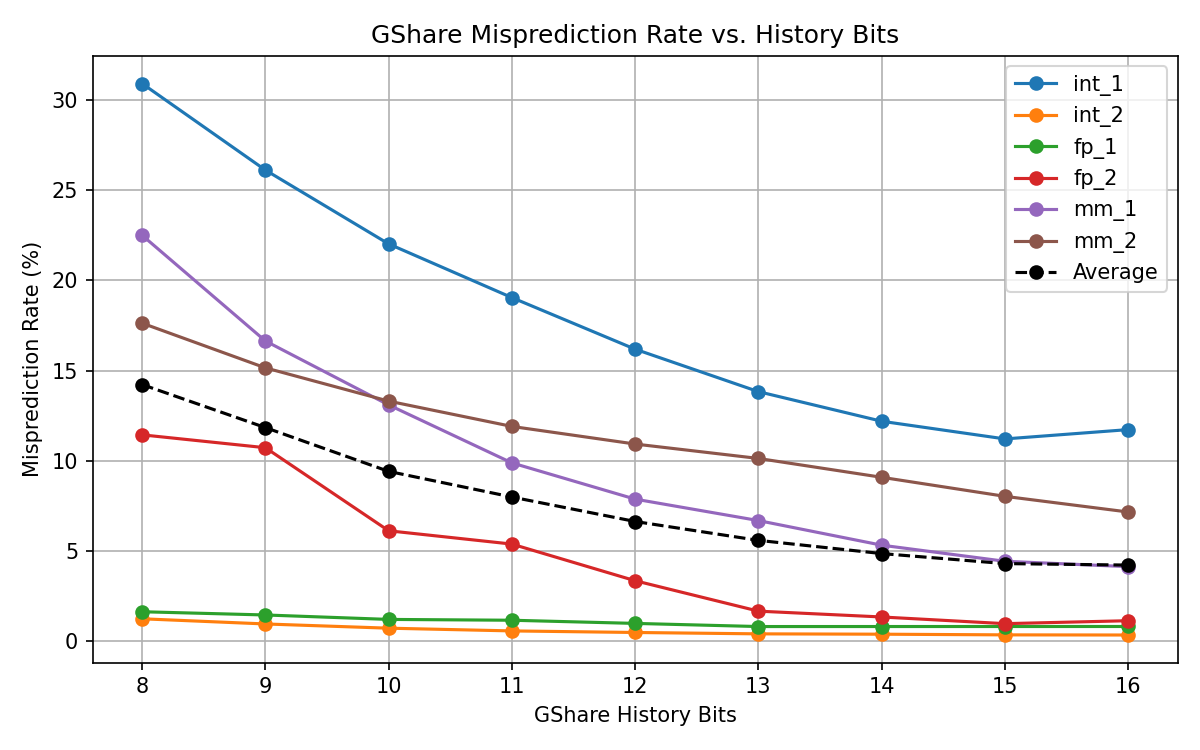
\includegraphics[width=0.65\textwidth]{gshare_sweep.png}
  \caption{G-Share Misprediction Rate vs. History Bits (8--16) for the Six Traces + Average}
  \label{fig:gshare_sweep}
\end{figure}

\begin{figure}[H]
  \centering
  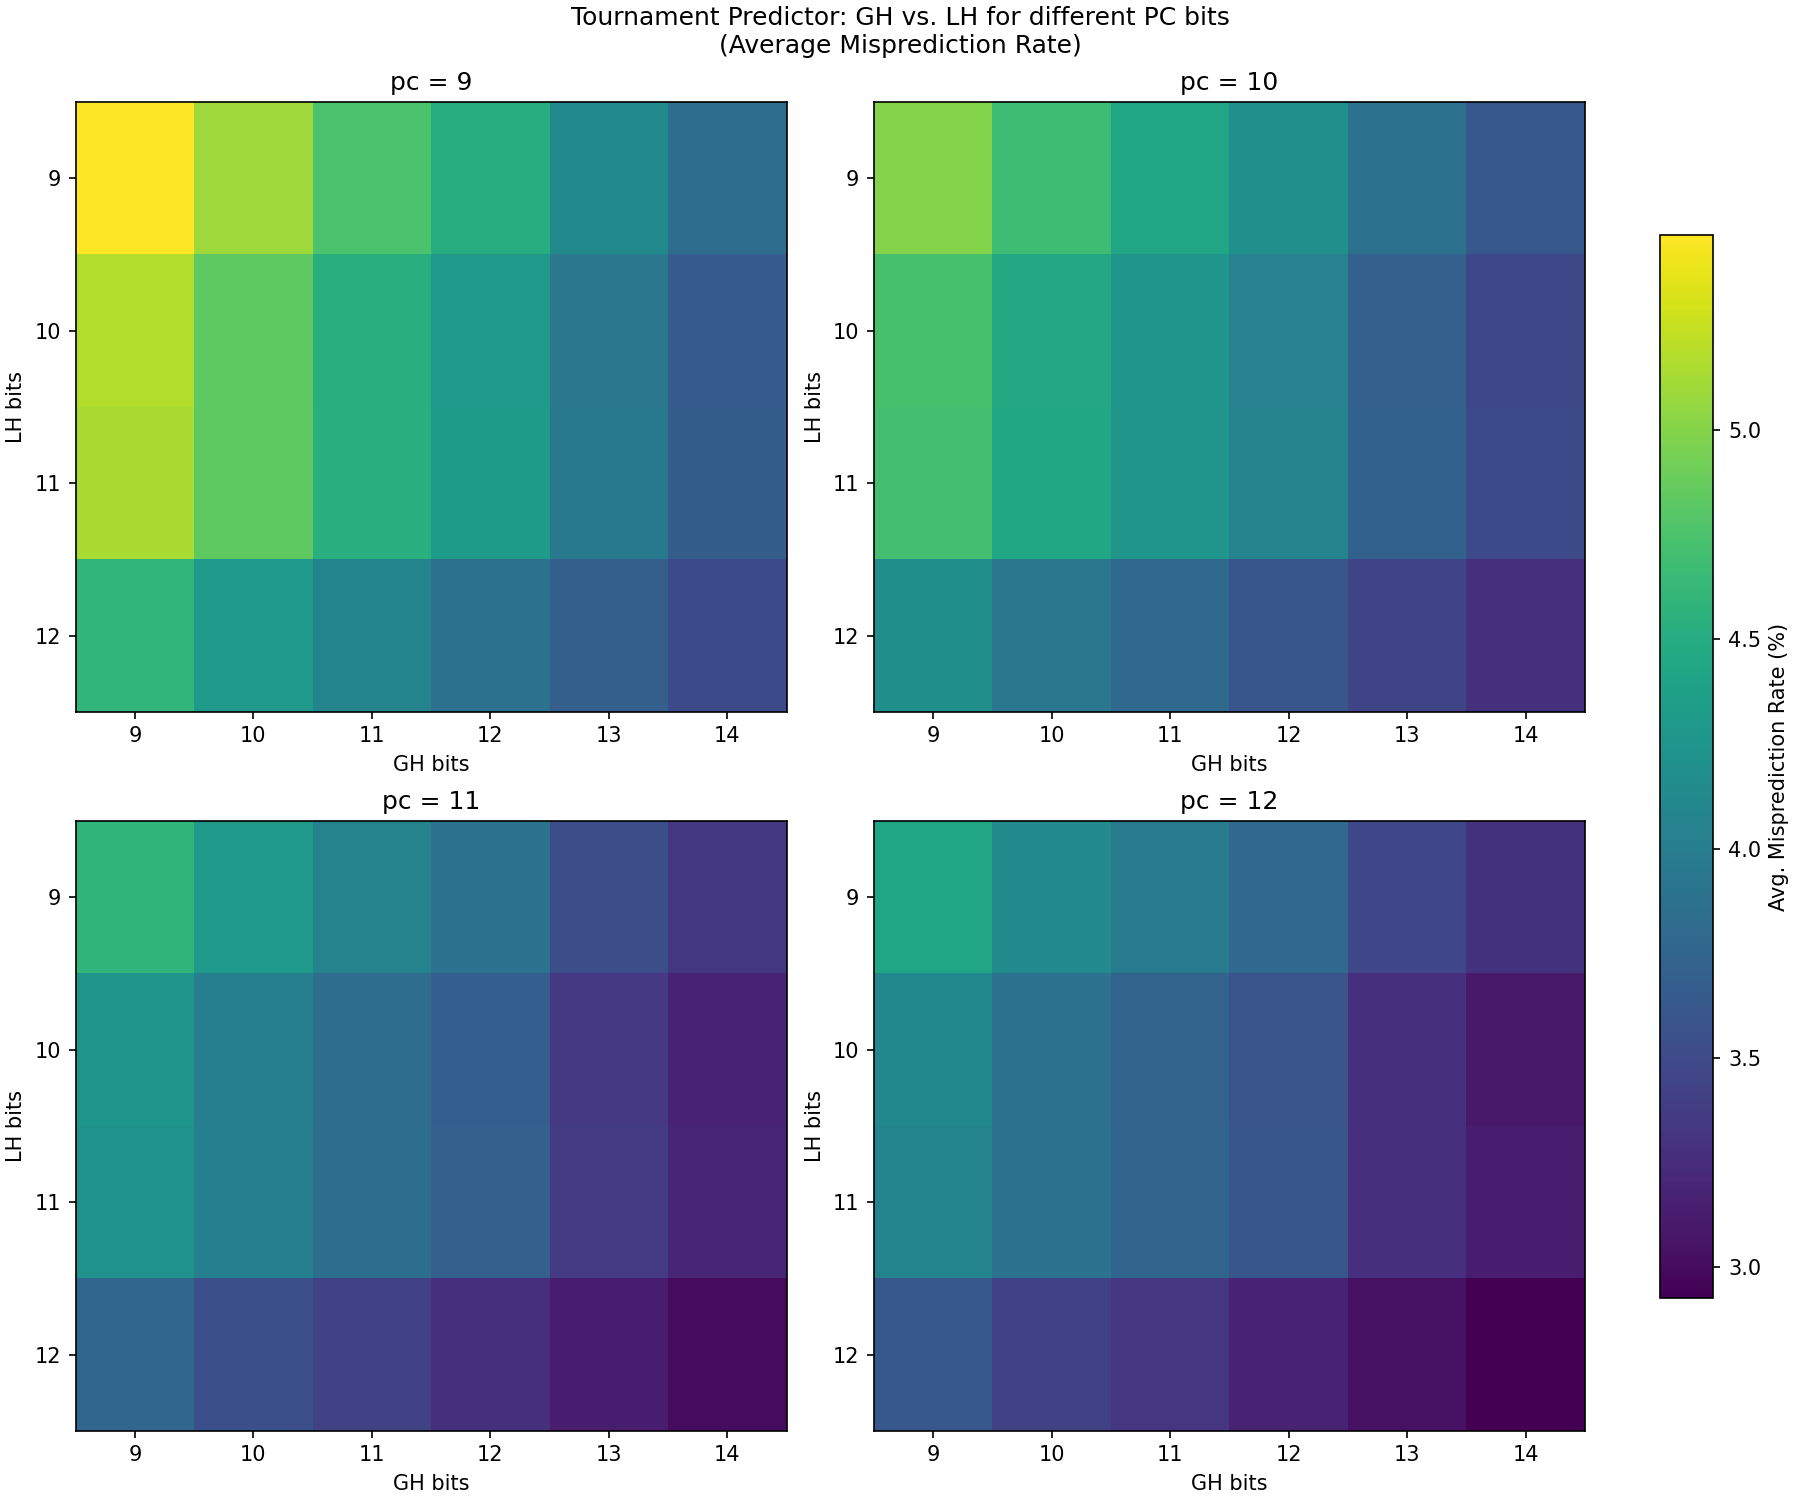
\includegraphics[width=0.8\textwidth]{tournament_heatmap.png}
  \caption{Tournament Predictor: GH vs. LH for Different PC Bits (Average Misprediction Rate)}
  \label{fig:tourn_heatmap}
\end{figure}

Overall, these sweeps reveal how increasing history length generally improves accuracy but also increases storage cost. In the tournament predictor heatmaps, \texttt{pcIndexBits} around 10--12 combined with moderate \texttt{ghistoryBits} and \texttt{lhistoryBits} can yield strong performance. The sweet spot in each subfigure often balances the trade-off between local and global correlation capture.

\section{Results and Conclusion}

\paragraph{Summary of Findings.}
\begin{itemize}
    \item TAGE outperforms simpler schemes in every tested scenario, though it uses more complex data structures.
    \item Tournament is a balanced design, typically besting G-Share, especially on memory-heavy traces.
    \item G-Share is a well-known baseline, relatively simple and fairly robust, but not as adaptive as Tournament or TAGE.
    \item Static is uniformly poor across the traces, highlighting the importance of dynamic branch prediction.
\end{itemize}

\paragraph{Future Work.}
\begin{itemize}
    \item \textbf{Perceptron or ML-based Branch Prediction:} Investigate neural methods.
    \item \textbf{Further TAGE Tuning:} Adjusting bank sizes, tags, or path history lengths for optimal coverage.
    \item \textbf{Hybrid Schemes:} Combine TAGE with other advanced predictors (e.g., loop predictors) to handle highly repetitive branches.
\end{itemize}

\section*{References}
\begingroup
\renewcommand{\section}[2]{}
\begin{thebibliography}{9}

\bibitem{yhsmith1981}
J.~Smith,
\newblock ``A Study of Branch Prediction Strategies,''
\newblock in \emph{ISCA '81: Proceedings of the 8th International Symposium on Computer Architecture}, 1981.
\newblock \url{https://courses.cs.washington.edu/courses/cse590g/04sp/Smith-1981-A-Study-of-Branch-Prediction-Strategies.pdf}

\bibitem{mcfarling1993combining}
S.~McFarling,
\newblock ``Combining Branch Predictors,''
\newblock \emph{WRL Technical Note TN-36}, Digital Equipment Corporation, 1993.
\newblock \url{https://www.ece.ucdavis.edu/~akella/270W05/mcfarling93combining.pdf}

\bibitem{seznec2006cottage}
A.~Seznec and P.~Michaud,
\newblock ``A Case for (Partially) TAgged GEometric History Length Branch Prediction,''
\newblock \emph{Journal of Instruction-Level Parallelism}, 2006.
\newblock \url{https://www.irisa.fr/caps/people/seznec/JILP-COTTAGE.pdf}

\bibitem{seznec2007tage}
A.~Seznec,
\newblock ``A 256Kbits L-TAGE Branch Predictor,''
\newblock \emph{Journal of Instruction-Level Parallelism}, 2007.
\newblock \url{https://www.irisa.fr/caps/people/seznec/L-TAGE.pdf}

\bibitem{seznec2011}
A.~Seznec,
\newblock ``TAGE-SC-L Branch Predictors Again,''
\newblock \emph{Journal of Instruction-Level Parallelism}, 2011.
\newblock \url{https://www.cs.cmu.edu/~18742/papers/Seznec2011.pdf}

\end{thebibliography}
\endgroup

\appendix
\section{Appendix: AI Tool Usage and Chat Logs}

\subsection{Overview}
In compliance with the project requirement to cite AI assistance and include prompts + outcomes, this appendix contains the key conversations with OpenAI’s ChatGPT (model gpt-4o). Below are excerpts showcasing how the tool was used to help debug code, generate example snippets, and provide explanatory text. All of these AI‐generated outputs were manually reviewed and substantially adapted.

\subsection{Conversation 1: TAGE predictor counter debug}

\begin{Verbatim}[fontsize=\tiny, breaklines=true]
Me: I have a partially implemented TAGE predictor in C code, but I'm running into an issue where the saturating counter for the tagged entries sometimes goes out of range. Could you help me debug this?

GPT-4o: Absolutely, I'd be glad to help you debug your TAGE predictor implementation! The saturating counter going out of range is usually caused by incorrect updates (like incrementing beyond the max or decrementing below zero) or initialization issues.

To dig into it properly, could you share:

1. The relevant code snippet for your **TAGE table entry structure**, especially the saturating counter part.
2. The part of the code where you **update** the saturating counters.
3. The defined **limits** for your saturating counters (e.g., are they 2-bit? 3-bit?).

With that info, I can pinpoint exactly where the issue is. In the meantime, here are a few things you can check right away:

---

### �� Quick Checks for Debugging

1. **Counter Saturation Boundaries**:
   Make sure you're checking boundaries before updating:
   ```c
   if (entry.counter < MAX_COUNTER) {
       entry.counter++;
   }
   ```
   and
   ```c
   if (entry.counter > MIN_COUNTER) {
       entry.counter--;
   }
   ```

2. **Bit-width Constants**:
   If your counters are, say, 3-bit (i.e., range -4 to 3 for signed, or 0 to 7 for unsigned), verify that:
   - You’re using the correct type (signed vs. unsigned).
   - Your increments/decrements respect the upper/lower limits.

3. **Initialization**:
   Counters should be initialized to a neutral state, typically 0 or mid-range.

4. **Sign Confusion**:
   Are you using a signed saturating counter and treating it like an unsigned one (or vice versa)?

---

If you're not sure where the issue is, paste the key sections of your code here, and I’ll help you trace it step by step.

Me: Yeah here's the code:

```
static inline void tage_train(uint32_t pc, uint8_t outcome) {
    int needAllocate = 0;
    if (primaryBank < NUM_BANKS) {
        int8_t pCtr = tageBank[primaryBank].entry[ bankGlobalIndex[primaryBank] ].saturateCounter;
        // If mispredicted and the sign of pCtr is opposite the actual outcome => might allocate
        if ((lastPrediction != outcome) && ((pCtr >= 0) != outcome)) {
            needAllocate = 1;
        }
    } else {
        needAllocate = (lastPrediction != outcome);
    }

    if (needAllocate) {
        int8_t minUse = 127;
        for (int i = 0; i < primaryBank; i++) {
            int8_t u = tageBank[i].entry[ bankGlobalIndex[i] ].usefulness;
            if (u < minUse) {
                minUse = u;
            }
        }
        if (minUse > 0) {
            for (int i = primaryBank - 1; i >= 0; i--) {
                // This might decrement usefulness too aggressively without bound checks
                tageBank[i].entry[ bankGlobalIndex[i] ].usefulness--;
            }
        } else {
            int Y = rand() & ((1 << (primaryBank - 1)) - 1);
            int X = primaryBank - 1;
            while ((Y & 1) != 0) {
                X--;
                Y >>= 1;
                if (X < 0) break;
            }
            for (int i = X; i >= 0; i--) {
                if (tageBank[i].entry[ bankGlobalIndex[i] ].usefulness == minUse) {
                    // Re-init but never resets saturateCounter properly
                    tageBank[i].entry[ bankGlobalIndex[i] ].tag = generateGlobalEntryTag(pc, i);
                    tageBank[i].entry[ bankGlobalIndex[i] ].saturateCounter =
                        (outcome == TAKEN) ? 2 : -2; // Wrong initial range
                    tageBank[i].entry[ bankGlobalIndex[i] ].usefulness = 0;
                    break;
                }
            }
        }
    }

    // Directly increment/decrement saturateCounter with no range checks
    if (primaryBank < NUM_BANKS) {
        if (outcome == TAKEN) {
            tageBank[primaryBank].entry[ bankGlobalIndex[primaryBank] ].saturateCounter++;
        } else {
            tageBank[primaryBank].entry[ bankGlobalIndex[primaryBank] ].saturateCounter--;
        }
    } else {
        // update Bimodal (incorrectly – no bounding)
        int idx = pc % BIMODAL_SIZE;
        if (outcome == TAKEN) {
            t_bimodalPredictor[idx]++;
        } else {
            t_bimodalPredictor[idx]--;
        }
    }

    // If primary != alternate, we update the primary’s usefulness if we used it
    // (again without bounding, which can go out of range)
    if (lastPrediction != alternatePrediction) {
        if (primaryBank < NUM_BANKS) {
            if (lastPrediction == outcome) {
                tageBank[primaryBank].entry[ bankGlobalIndex[primaryBank] ].usefulness++;
            } else {
                tageBank[primaryBank].entry[ bankGlobalIndex[primaryBank] ].usefulness--;
            }
        }
    }

    // Shift in new outcome
    for (int i = MAX_HISTORY_LEN - 1; i > 0; i--) {
        t_globalHistory[i] = t_globalHistory[i - 1];
    }
    t_globalHistory[0] = outcome ? TAKEN : NOTTAKEN;

    // Update path history
    t_pathHistory <<= 1;
    t_pathHistory += (pc & 1);
    t_pathHistory &= ((1 << 16) - 1);

    // Update compressed histories (but missing some checks or re-initializations)
    for (int i = 0; i < NUM_BANKS; i++) {
        t_updateCompressed(&tageBank[i].indexCompressed, t_globalHistory);
        t_updateCompressed(&tageBank[i].tagCompressed[0], t_globalHistory);
        t_updateCompressed(&tageBank[i].tagCompressed[1], t_globalHistory);
    }
}
```

GPT-4o: Below is a rundown of what’s causing your **saturating counters** to go out of range in the snippet you posted and how to fix it. The main issues are:

1. **No Bound Checks** when incrementing or decrementing the saturating counters.
2. **Re-initialization Values** (`+2` or `-2`) that may be inconsistent with the defined bit width of your counters.
3. **Usefulness Counters** also updated without bounding, which can similarly wrap around.

Let’s walk through the details.

---

## 1. Missing Bound Checks in Saturating Counter Updates

Right now, you do:
```c
if (outcome == TAKEN) {
    tageBank[primaryBank].entry[ bankGlobalIndex[primaryBank] ].saturateCounter++;
} else {
    tageBank[primaryBank].entry[ bankGlobalIndex[primaryBank] ].saturateCounter--;
}
```
with no checks. If you keep incrementing, you eventually push `saturateCounter` above the intended maximum; likewise, repeated decrementing can push it below the minimum. In an `int8_t`, once it passes `+127` or below `-128`, it wraps around, and your predictor logic breaks.

### **How to Fix**

1. **Decide the width** of your counters. Commonly in TAGE, each tagged entry uses a **3-bit** or **4-bit** signed saturating counter. For instance, if you use a **3-bit** scheme with sign-based prediction:
   - Negative values (−4 to −1) => “predict not taken”
   - Zero or positive (0 to +3) => “predict taken”
   - And you saturate at **−4** (min) or **+3** (max).

2. **Clamp** on increment/decrement. For example, if using a 3-bit range of `-4..+3`:
   ```c
   #define MAX_CNT  3   // +3 is the maximum
   #define MIN_CNT -4   // -4 is the minimum

   int8_t *ctr = &tageBank[primaryBank].entry[ bankGlobalIndex[primaryBank] ].saturateCounter;
   if (outcome == TAKEN) {
       if (*ctr < MAX_CNT) {
           (*ctr)++;
       }
   } else {
       if (*ctr > MIN_CNT) {
           (*ctr)--;
       }
   }
   ```

That way, the counter does not exceed +3 or drop below −4, ensuring proper saturating behavior.

---

## 2. Re-Initializing the Counter to +2 or −2

Inside your “allocate” path, you do:
```c
tageBank[i].entry[ bankGlobalIndex[i] ].saturateCounter =
    (outcome == TAKEN) ? 2 : -2;  // Wrong initial range if 2-bit or mismatch
```
This can be **fine** if your saturating counter range is at least ±2. (In a 3-bit scheme from −4..+3, ±2 is valid and comfortably within the range.) However, if you intended to use only **2 bits** with sign-based logic, then the range is typically −2..+1 (four total states), and +2 would already be “out of range.”

### **How to Fix**

- Confirm your desired saturating counter width and sign convention.
- If it’s 3 bits (−4..+3), re-initializing to ±2 is perfectly valid. Just make sure your bounding constants match.
- If it’s 2 bits (−2..+1), then you must clamp `+2` or `-2` to that narrower range.

---

## 3. No Bound Checks for Usefulness Counters

You also have a “usefulness” field:
```c
// This might decrement usefulness too aggressively without bound checks
tageBank[i].entry[ bankGlobalIndex[i] ].usefulness--;
```
and later:
```c
if (lastPrediction == outcome) {
    tageBank[primaryBank].entry[ bankGlobalIndex[primaryBank] ].usefulness++;
} else {
    tageBank[primaryBank].entry[ bankGlobalIndex[primaryBank] ].usefulness--;
}
```
If `usefulness` is supposed to be a small saturating counter (e.g., 2 bits or 3 bits), it can **wrap around** the same way as `saturateCounter`.

### **How to Fix**

- Decide the max/min for `usefulness` (e.g., 0..3).
- Clamp it in exactly the same way:
  ```c
  #define U_MAX 3
  #define U_MIN 0

  if (tageBank[i].entry[ bankGlobalIndex[i] ].usefulness > U_MIN) {
      tageBank[i].entry[ bankGlobalIndex[i] ].usefulness--;
  }

  // Similarly for increment.
  ```

---

## 4. Bimodal Updates

In your bimodal branch:
```c
if (outcome == TAKEN) {
    t_bimodalPredictor[idx]++;
} else {
    t_bimodalPredictor[idx]--;
}
```
If `t_bimodalPredictor[idx]` is also a saturating counter (commonly 2 bits or 3 bits in a bimodal table), you must do the same saturating logic here:
```c
if (outcome == TAKEN) {
    if (t_bimodalPredictor[idx] < MAX_BIMODAL) {
        t_bimodalPredictor[idx]++;
    }
} else {
    if (t_bimodalPredictor[idx] > MIN_BIMODAL) {
        t_bimodalPredictor[idx]--;
    }
}
```

---

## Putting It All Together

**Key actions** to fix the out-of-range saturating counter bug:

1. **Define constants** for the saturating counter bounds.
2. **Clamp** each increment/decrement to those bounds.
3. Ensure your **initial values** (like +2 or −2) fall within the same bounds.
4. Do the same for the **usefulness** counters and bimodal counters (if they’re also meant to be saturating).

Once you add those fixes, you shouldn’t see the counters blowing past the valid range. Let me know if you have other questions on TAGE details, or if you need help deciding on the bit widths for your counters!
\end{Verbatim}

\subsection{Conversation 2: TAGE Predictor Overview}
\begin{Verbatim}[fontsize=\tiny, breaklines=true]
Me: Please provide a high-level explanation of how a TAGE predictor works, focusing on the multi-bank structure, the geometric history lengths, and how partial tags are generated.

GPT-4o: Sure! Here's a high-level explanation of how a **TAGE (TAgged GEometric history length) predictor** works, with a focus on its **multi-bank structure**, **geometric history lengths**, and **partial tag generation**:

---

### �� Overview of TAGE

TAGE is a **state-of-the-art branch predictor** used in modern CPUs to guess the direction of branches (taken or not taken) before they're resolved, improving instruction-level parallelism. It builds on the idea that **longer branch histories** can improve prediction accuracy, but in a smart and scalable way.

---

### �� Multi-bank Structure

- TAGE uses **multiple predictor components**, often called **banks or tables**.
- Each table (except for the base one) is associated with a **different history length**, forming a hierarchy.
- The predictor uses **one base predictor** (often a simple bimodal predictor) and several **tagged predictor tables**.
- Each tagged table is indexed using a **compressed version** of the global branch history, allowing it to capture correlations over different history lengths.

**Key idea**: If a long history length yields a confident prediction, use it. Otherwise, fall back to shorter histories or the base predictor.

---

### �� Geometric History Lengths

- Each tagged table uses a **different history length**, forming a **geometric progression**:
  ```
  L(i) = floor(α^i), for i = 0 to N-1
  ```
  where:
  - `L(i)` is the history length for table `i`
  - `α` is a geometric growth factor (e.g., 1.5 to 2)
  - `N` is the number of tagged tables
- This setup allows TAGE to cover a wide range of history lengths with **fewer tables**, efficiently balancing coverage and resource usage.

---

### �� Partial Tag Generation

- Each entry in a tagged table stores a **partial tag** to match against the branch’s history-derived signature.
- A **partial tag** is generated by:
  - **Hashing or folding** the program counter (PC) and the global history into a small number of bits.
  - This allows a small tag to identify whether a prediction entry corresponds to the current branch and history pattern.
- Partial tags help **differentiate between branches** that may map to the same table entry (avoiding aliasing errors).

---

### �� Prediction Process

1. For a given branch:
   - The PC and global history are used to index all tables.
   - The predictor searches for the **longest history match** among the tables.
2. If a match is found (tag matches), the prediction from that table is used.
3. If no match, the base predictor is used.
4. If two or more matches exist, the **longest matching history** wins.

---

### ✅ Summary

- **Multi-bank structure**: Multiple tables store predictions with varying history lengths.
- **Geometric history lengths**: History lengths grow exponentially to capture both short-term and long-term correlations.
- **Partial tags**: Small hash-like signatures identify valid entries for a given PC/history pair.

Let me know if you want a diagram or a more detailed example to go with this!
\end{Verbatim}

\subsection{Conversation 3: TAGE predictor bit calculation}
\begin{Verbatim}[fontsize=\tiny, breaklines=true]
Me: I'm trying to keep my TAGE predictor under 64K + 256 bits. How do I calculate the bit usage for each bank if I have 3 bits for the saturating counter, 10 bits for the tag, and 2 or 3 bits for usefulness? Also, how do I account for compressed histories?

GPT-4o: Great question! Let's break this down and calculate the storage used per entry in each TAGE bank, and then look at how to stay within your budget of **64K + 256 bits** (which is **65,280 bits** total).

---

### �� **Per-Entry Bit Usage (per bank)**

For **each TAGE predictor bank entry**, you typically store:

1. **Tag** = 10 bits
2. **Saturating Counter** = 3 bits
3. **Usefulness Counter** = 2 or 3 bits (depends on your design)

So per entry:
- If 2-bit usefulness: `10 + 3 + 2 = 15 bits`
- If 3-bit usefulness: `10 + 3 + 3 = 16 bits`

---

### �� **Compressed Histories**

**Compressed histories** are used to save storage on the history-based indexing and tagging functions. These aren't per-entry — they’re global/shared across banks.

- You typically store a **compressed history** for each bank, used in indexing and tagging. The size of each compressed history depends on:
  - The global history length used
  - Number of banks
  - The folding strategy

In many designs, each compressed history is ~10–16 bits per component (depending on folding), and you may have:
- One for index generation (per bank)
- One for tag generation (per bank)

So rough estimate:
`~2 compressed histories × N banks × ~16 bits = small amount`
Say for 8 banks: `2 × 8 × 16 = 256 bits` — which actually matches the **+256** in your `64K + 256` constraint.

�� **Conclusion:** You’re allowed to spend **64K bits (65,024 bits)** on your *tables*, and the extra 256 bits are for compressed histories.

---

### ✅ **Storage Budget Summary**

You have:
- **64K bits = 65,024 bits for TAGE entries**
- **+256 bits for compressed histories**

Let’s calculate how many entries you can have per bank.

---

### �� **Example: How Many Entries per Bank?**

Let’s say:
- 4 banks
- Usefulness counter = 2 bits
- So each entry = 15 bits

Assuming equal size per bank:
```
Total bits per bank = 65,024 / 4 = 16,256 bits
Entries per bank = 16,256 / 15 ≈ 1,083 entries
```

If usefulness = 3 bits (16 bits per entry):
```
Entries per bank = 16,256 / 16 = 1,016 entries
```

You can also vary the number of entries per bank (fewer entries for longer-history banks).

---

### ��️ Other Considerations:

- **Base Predictor**: Don’t forget that TAGE usually includes a base predictor (like a bimodal table), which may need separate bits.
- **Banked vs Fully Associative**: If you implement associativity or partial associativity, it affects indexing and possibly tag size.
- **Replacement Information**: If you store any replacement priority bits, you’ll need to include those too.

---

### TL;DR:

- **Per-entry size = tag (10) + ctr (3) + useful (2–3) = 15–16 bits**
- **Compressed histories ≈ 256 bits total — fits within the “+256 bits” budget**
- Use your total bit budget (65,024) to divide across banks and determine entry count

Let me know how many banks you’re using or if you want help optimizing your layout!
\end{Verbatim}

\subsection{Conversation 4: TAGE Training Function Annotation}
\begin{Verbatim}[fontsize=\tiny, breaklines=true]
Me:

Could you annotate the tage_train() function?

static inline void tage_train(uint32_t pc, uint8_t outcome) {
    int needAllocate = 0;
    if (primaryBank < NUM_BANKS) {
        int8_t pCtr = tageBank[primaryBank].entry[ bankGlobalIndex[primaryBank] ].saturateCounter;
        // If mispredicted and the sign of pCtr is opposite the actual outcome => might allocate
        if ((lastPrediction != outcome) && ((pCtr >= 0) != outcome)) {
            needAllocate = 1;
        }
    } else {
        needAllocate = (lastPrediction != outcome);
    }

    if (needAllocate) {
        int8_t minUse = 127;
        for (int i = 0; i < primaryBank; i++) {
            int8_t u = tageBank[i].entry[ bankGlobalIndex[i] ].usefulness;
            if (u < minUse) {
                minUse = u;
            }
        }
        if (minUse > 0) {
            for (int i = primaryBank - 1; i >= 0; i--) {
                tageBank[i].entry[ bankGlobalIndex[i] ].usefulness--;
            }
        } else {
            int Y = rand() & ((1 << (primaryBank - 1)) - 1);
            int X = primaryBank - 1;
            while ((Y & 1) != 0) {
                X--;
                Y >>= 1;
                if (X < 0) break;
            }
            for (int i = X; i >= 0; i--) {
                if (tageBank[i].entry[ bankGlobalIndex[i] ].usefulness == minUse) {
                    // Re-init
                    tageBank[i].entry[ bankGlobalIndex[i] ].tag = generateGlobalEntryTag(pc, i);
                    tageBank[i].entry[ bankGlobalIndex[i] ].saturateCounter =
                        (outcome == TAKEN) ? 0 : -1;
                    tageBank[i].entry[ bankGlobalIndex[i] ].usefulness = 0;
                    break;
                }
            }
        }
    }

    // Update the saturating counter
    if (primaryBank < NUM_BANKS) {
        updateSaturate(
            &tageBank[primaryBank].entry[ bankGlobalIndex[primaryBank] ].saturateCounter,
            outcome,
            LEN_COUNTS
        );
    } else {
        // update Bimodal
        int idx = pc % BIMODAL_SIZE;
        updateSaturateMinMax(&t_bimodalPredictor[idx], outcome, 0, (1 << LEN_BIMODAL) - 1);
    }

    // If primary != alternate, we update the primary’s usefulness if we used it
    if (lastPrediction != alternatePrediction) {
        if (primaryBank < NUM_BANKS) {
            updateSaturateMinMax(
                &tageBank[primaryBank].entry[ bankGlobalIndex[primaryBank] ].usefulness,
                (lastPrediction == outcome),
                0, 3
            );
        }
    }

    // Shift in new outcome
    for (int i = MAX_HISTORY_LEN - 1; i > 0; i--) {
        t_globalHistory[i] = t_globalHistory[i - 1];
    }
    t_globalHistory[0] = outcome ? TAKEN : NOTTAKEN;

    // Update path history
    t_pathHistory <<= 1;
    t_pathHistory += (pc & 1);
    t_pathHistory &= ((1 << 16) - 1);

    // Update compressed histories
    for (int i = 0; i < NUM_BANKS; i++) {
        t_updateCompressed(&tageBank[i].indexCompressed, t_globalHistory);
        t_updateCompressed(&tageBank[i].tagCompressed[0], t_globalHistory);
        t_updateCompressed(&tageBank[i].tagCompressed[1], t_globalHistory);
    }
}

GPT-4o: Below is an annotated version of the `tage_train()` function. The annotations are placed as comments before or alongside relevant sections of the code to explain the purpose and logic behind each step.

---

```cpp
static inline void tage_train(uint32_t pc, uint8_t outcome) {
    // 1. Determine whether we need to allocate a new entry in the TAGE tables (i.e., whether
    //    the prediction was mispredicted and we have reason to believe a new entry could
    //    improve future prediction accuracy).

    int needAllocate = 0;

    // primaryBank is the TAGE bank (or set of banks) that provided the final prediction.
    // If primaryBank is valid (less than NUM_BANKS), we have a prediction from TAGE.
    // Otherwise, the prediction came from the bimodal predictor.
    if (primaryBank < NUM_BANKS) {
        // pCtr is the saturating counter from the TAGE table entry in the primary bank.
        int8_t pCtr = tageBank[primaryBank].entry[ bankGlobalIndex[primaryBank] ].saturateCounter;

        // If the final prediction was wrong AND the sign of pCtr is opposite from the actual outcome,
        // we may want to allocate a new entry from the other TAGE banks (which didn't match).
        // This is a typical "allocate on misprediction" strategy for TAGE.
        if ((lastPrediction != outcome) && ((pCtr >= 0) != outcome)) {
            needAllocate = 1;
        }
    } else {
        // If the prediction was from the bimodal predictor, we consider allocating
        // if the prediction was simply incorrect.
        needAllocate = (lastPrediction != outcome);
    }

    // 2. If we need to allocate, determine whether it is possible or desirable to do so.
    //    TAGE banks use a "usefulness" counter to decide if an entry is worth replacing.

    if (needAllocate) {
        int8_t minUse = 127;

        // Search for the minimum "usefulness" across all banks that are more selective (i.e. < primaryBank).
        // The lower this value, the more likely it is that an entry can be replaced.
        for (int i = 0; i < primaryBank; i++) {
            int8_t u = tageBank[i].entry[ bankGlobalIndex[i] ].usefulness;
            if (u < minUse) {
                minUse = u;
            }
        }

        // If all banks have high usefulness, we decrement the usefulness counters (to give a chance
        // for entries to become less useful and thus replaceable in the future).
        if (minUse > 0) {
            for (int i = primaryBank - 1; i >= 0; i--) {
                tageBank[i].entry[ bankGlobalIndex[i] ].usefulness--;
            }
        } else {
            // Otherwise, at least one bank has minimal usefulness, and we can replace an entry in one of
            // those banks with a new tag/saturating counter.

            // Y is used here to randomly select which bank (among the possible ones) gets the new entry.
            // The expression "(1 << (primaryBank - 1)) - 1" essentially creates a bitmask.
            // For example, if primaryBank = 3, we get (1 << 2) - 1 = 3 (binary 11).
            int Y = rand() & ((1 << (primaryBank - 1)) - 1);
            int X = primaryBank - 1;

            // This loop steps backward through the banks (less selective to more selective) until it
            // finds one that is randomly selected to allocate.
            while ((Y & 1) != 0) {
                X--;
                Y >>= 1;
                if (X < 0) break;
            }

            // Once we choose bank X, look for an entry in that bank with usefulness == minUse.
            // We then re-initialize it with the new tag, a saturating counter biased by the outcome,
            // and reset usefulness.
            for (int i = X; i >= 0; i--) {
                if (tageBank[i].entry[ bankGlobalIndex[i] ].usefulness == minUse) {
                    // Re-initialize the entry with the new tag and starting counter value.
                    tageBank[i].entry[ bankGlobalIndex[i] ].tag = generateGlobalEntryTag(pc, i);
                    tageBank[i].entry[ bankGlobalIndex[i] ].saturateCounter =
                        (outcome == TAKEN) ? 0 : -1;
                    tageBank[i].entry[ bankGlobalIndex[i] ].usefulness = 0;
                    break;
                }
            }
        }
    }

    // 3. Update the saturating counter in the primary bank (if used), or the bimodal predictor (otherwise).
    //    Saturating counters move up/down based on whether the outcome was TAKEN or NOTTAKEN.
    if (primaryBank < NUM_BANKS) {
        updateSaturate(
            &tageBank[primaryBank].entry[ bankGlobalIndex[primaryBank] ].saturateCounter,
            outcome,
            LEN_COUNTS
        );
    } else {
        // If the prediction came from the bimodal predictor, update it instead.
        int idx = pc % BIMODAL_SIZE;
        updateSaturateMinMax(&t_bimodalPredictor[idx], outcome, 0, (1 << LEN_BIMODAL) - 1);
    }

    // 4. If the primary prediction was different from the alternate prediction,
    //    update the usefulness counter for the primary table’s entry. We reward or penalize
    //    the primary TAGE entry if it got the actual outcome right or wrong, respectively.
    if (lastPrediction != alternatePrediction) {
        if (primaryBank < NUM_BANKS) {
            updateSaturateMinMax(
                &tageBank[primaryBank].entry[ bankGlobalIndex[primaryBank] ].usefulness,
                (lastPrediction == outcome),
                0, 3
            );
        }
    }

    // 5. Update the global history with the new outcome. This shifts the array t_globalHistory
    //    and inserts the latest taken/not-taken result at the front (index 0).
    for (int i = MAX_HISTORY_LEN - 1; i > 0; i--) {
        t_globalHistory[i] = t_globalHistory[i - 1];
    }
    t_globalHistory[0] = outcome ? TAKEN : NOTTAKEN;

    // Update the path history (which often tracks the program-counter's least significant bits).
    t_pathHistory <<= 1;
    t_pathHistory += (pc & 1);
    t_pathHistory &= ((1 << 16) - 1); // keep only the lower 16 bits

    // 6. Update the compressed histories for each TAGE bank. Compressed history is used to index
    //    and tag TAGE tables with partial, hashed versions of the global history.
    for (int i = 0; i < NUM_BANKS; i++) {
        t_updateCompressed(&tageBank[i].indexCompressed, t_globalHistory);
        t_updateCompressed(&tageBank[i].tagCompressed[0], t_globalHistory);
        t_updateCompressed(&tageBank[i].tagCompressed[1], t_globalHistory);
    }
}
```

### Summary of Key Points

1. **`needAllocate`:** Determines if the predictor will attempt to allocate a new entry in TAGE for better prediction in the future. This is triggered by a misprediction and a sign mismatch between the saturating counter and the actual outcome.

2. **Usefulness Counters:** TAGE uses “usefulness” to determine if an entry is likely still relevant. If no entries can be replaced (i.e., all have high usefulness), the predictor decrements usefulness counters to eventually free them for re-allocation.

3. **Random Replacement Among Candidates:** If multiple entries are at minimum usefulness, TAGE randomly chooses which one to replace. This helps spread out the chance of finding a beneficial new entry.

4. **Updating Saturating Counters:** After each prediction, the saturating counter is updated to reflect the actual outcome, so the same pattern in the future can be predicted more accurately.

5. **Usefulness Update:** If the primary TAGE bank disagreed with the alternate but was correct, we increase its usefulness (and vice versa).

6. **Updating History:** Global history (`t_globalHistory`), path history (`t_pathHistory`), and compressed history are all updated with the latest outcome to keep the TAGE tables properly indexed and tagged for future predictions.
\end{Verbatim}

\subsection{Conversation 5: Docker setup for predictor}
\begin{Verbatim}[fontsize=\tiny, breaklines=true]
Me: Show me how to set up a Docker container to compile and run `predictor.c` with `make`. I'm on Windows, so I might need the correct volume mounts. Also show me the exact commands I'd run to test the .bz2 trace files in my trace/ dir.

GPT-4o: Sure! Let's walk through setting up a Docker container that compiles and runs `predictor.c` using `make`, and also lets you test `.bz2` trace files from a `trace/` directory on your Windows machine.

---

## ✅ Step 1: Project Layout (Assumed)

Suppose your project folder looks like this on your **Windows host**:

```
C:\Users\YourName\branch_predictor\
│
├── predictor.c
├── Makefile
├── sim
├── trace\
│   ├── trace1.bz2
│   └── trace2.bz2
```

We'll mount this directory into Docker.

---

## ✅ Step 2: Create a Dockerfile (optional)

If you want a custom environment, create a `Dockerfile` like this:

```Dockerfile
FROM ubuntu:22.04

# Install build tools and bunzip2
RUN apt update && apt install -y build-essential bzip2

WORKDIR /app
```

Build it with:

```bash
docker build -t predictor-env .
```

Alternatively, you can skip this and use a base image like `gcc` with bzip2.

---

## ✅ Step 3: Run Docker with Proper Mounts

On **Windows**, your path `/mnt/c/Users/YourName/branch_predictor` corresponds to `C:\Users\YourName\branch_predictor`.

Here’s the Docker run command:

```bash
docker run --rm -it -v /mnt/c/Users/YourName/branch_predictor:/app -w /app predictor-env bash
```

Or, if you didn’t build a custom image:

```bash
docker run --rm -it -v /mnt/c/Users/YourName/branch_predictor:/app -w /app ubuntu:22.04 bash
```

Then install the tools inside the container:

```bash
apt update
apt install -y build-essential bzip2
```

---

## ✅ Step 4: Compile with Make

Inside the container (you're now at `/app`, which is your Windows project dir):

```bash
make
```

This should compile `predictor.c` into the binary `sim`.

---

## ✅ Step 5: Run Sim with `.bz2` Trace Files

Assuming `sim` takes a trace file as argument like this:

```bash
./sim -t trace/trace1.bz2
```

You can run any of the traces like:

```bash
./sim -t trace/trace1.bz2
./sim -t trace/trace2.bz2
```

If you want to loop over them:

```bash
for f in trace/*.bz2; do
  ./sim -t "$f"
done
```

---

## �� Full Session Recap (All Together)

```bash
docker run --rm -it -v /mnt/c/Users/YourName/branch_predictor:/app -w /app ubuntu:22.04 bash

# In Docker:
apt update
apt install -y build-essential bzip2
make
./sim -t trace/trace1.bz2
```

---

Would you like help writing a `Makefile`, if you don't already have one? Or a script to automate all trace testing?
\end{Verbatim}

\subsection{Conversation 6: Gshare Misprediction Rate Difference}
\begin{Verbatim}[fontsize=\tiny, breaklines=true]
Me: Can you explain why the runall.sh script outputs "Misprediction Rate: 0.826" for gshare:14 on fp_1 but "Misprediction Rate: 0.827" for gshare:15? Are those differences from random seeds or actual structural differences in the table indexing?

GPT-4o: The slight difference in **Misprediction Rate** between `gshare:14` (0.826) and `gshare:15` (0.827) is most likely due to **actual structural differences in the indexing mechanism** of the **gshare** predictor, rather than random seeds — assuming the simulator is deterministic (most academic simulators are).

Let me break it down for you:

---

### �� What is gshare?

**gshare** is a dynamic branch predictor that uses:

- **Global History Register (GHR)**: tracks outcomes of recent branches.
- **Program Counter (PC)**: identifies the current branch.
- These two are XOR’ed together to generate an **index** into a **prediction table** (Pattern History Table or PHT).

---

### �� What does `gshare:14` or `gshare:15` mean?

These likely refer to the number of **index bits** used to access the prediction table:
- `gshare:14` → 14 bits are used to index the table.
- `gshare:15` → 15 bits are used.

This affects:
- **Table size** (2¹⁴ vs. 2¹⁵ entries).
- **Indexing behavior**, because more bits from the PC and GHR are used in the XOR.

---

### �� Why the slight difference?

1. **Structural behavior:**
   - A larger table (`gshare:15`) generally helps — more entries, less aliasing.
   - But it can also cause **different aliasing patterns**: more bits from the GHR and PC are involved, and the way they XOR may group branches differently.
   - This can cause **some branches to benefit** and others to suffer, especially on specific traces like `fp_1`.

2. **Trace sensitivity:**
   - The `fp_1` trace might have branch patterns that align better with 14 bits than 15 due to its structure or frequency of certain PCs.

3. **Rounding error?**
   - If the misprediction rate is output as a **rounded float**, e.g. 0.826 vs. 0.827, the actual raw numbers might be very close, like:
     - `0.8264` (rounded to 0.826)
     - `0.8265` (rounded to 0.827)

---

### �� Is randomness involved?

Unlikely unless:
- The simulator is non-deterministic (e.g., uses random initial table values or thread interleaving).
- You’re using randomized inputs or seeds (e.g., in a neural predictor or ML-based branch predictor — not typical for gshare).

If you're using a standard gshare implementation and always run the same trace (`fp_1`), the results should be deterministic.

---

### ✅ Summary:

The difference in misprediction rate between `gshare:14` and `gshare:15` is due to **structural indexing differences** (how GHR and PC bits XOR to select table entries), not randomness. The slightly worse rate for `gshare:15` on `fp_1` is probably a quirk of **aliasing patterns** or rounding precision — not an anomaly.

If you want, I can show you how to visualize the indexing to see exactly which bits are used at each size.
\end{Verbatim}

\thispagestyle{ack_footer}

\end{document}
